\apendice{Documentación de usuario}

\section{Introducción}

A lo largo de este apéndice vamos a indicar el material necesario para poder ejecutar el proyecto, así como la manera de instalarlo y hacerlo funcionar una vez contemos con todos los elementos requeridos.

\section{Requisitos de usuarios}

\subsection{Requisitos software}\label{sec:ReqSoftware}

A continuación se muestra una lista de todos los requisitos mínimos para la ejecución del proyecto. En las secciones \ref{sec:Instalacion} y \ref{sec:InstalacionOpcional} podrá encontrarse el método de instalación para cada uno de estos componentes.

Podemos advertir diferentes distribuciones (ver sección \ref{subsec:distribuciones}) y diferentes maneras de ejecutar el proyecto (ver sección \ref{sec:manualUsuario}), por lo que no todos los componentes son necesarios en todos los casos

\begin{itemize}
\item Java 8
\item Apache Maven (Solo necesario si requerimos Apache Spark)
\item Apache Spark (Solo necesario si deseamos lanzar las ejecuciones en nuestra máquina)
\end{itemize}

\subsection{Requisitos mínimos del sistema}

Dado que existen diferentes modos de uso del proyecto, es necesario indicar aquí varias configuraciones:

\begin{itemize}
\item Únicamente deseamos generar un archivo .zip para nuestro proyecto:
	\begin{itemize}
	\item \textbf{Procesador:} Pentium 2 266 MHz \cite{minRequerimentsJava}
	\item \textbf{Memoria RAM:} 128MB \cite{minRequerimentsJava}
	\item \textbf{Espacio libre en disco:} aprox. 180 MB + Espacio adicional para los conjuntos de datos.
	\end{itemize}
\item Deseamos ejecutar los algoritmos en nuestro proyecto:
	\begin{itemize}
	\item \textbf{Procesador:} Procesador multihilo con capacidad de soportar, al menos, 2 hilos simultaneamente.
	\item \textbf{Memoria RAM:} 4 GB
	\item \textbf{Espacio libre en disco:} aprox 2.1GB más el espacio adicional para los conjuntos de datos que deseemos almacenar.
	\end{itemize}
\end{itemize}

Quede constancia, además de los requisitos mencionados, que hay que tener en cuenta dos aspectos más:
\begin{itemize}
\item La memoria mínima que un ejecutor de Spark puede tener es 1 GB. Por lo tanto, tal vez sea necesario ajustar el número de ejecutores si no tenemos memoria suficiente.
\item Los requisitos definidos para la ejecución de Spark en ningún caso se van a parecer a los usados en una ejecución ``real'' en un clúster, cuyos requisitos recomendados pueden encontrarse en la página oficial de Spark \cite{requisitosSpark}.
\end{itemize}


\section{Instalación}\label{sec:Instalacion}

A continuación se van a definir los métodos de instalación de todos los componentes necesarios para ejecutar el proyecto, de cara a facilitar el mantenimiento en futuras versiones de la biblioteca y permitir la instalación al usuario.

Estos métodos de instalación hacen referencia a la instalación en máquinas con un sistema operativo basado en alguna distribución de Debian. En nuestro caso, esta distribución ha sido Ubuntu 14.04.

\subsection{Oracle Java 8}

Aunque existen distribuciones libres de Java, usaremos la que proporciona Oracle (\url{http://www.java.com}) por el hecho de que incluye una serie de programas que pueden usarse para medir el rendimiento de aplicaciones Java (JConsole y JVisualVM). Cualquier otra distribución será igualmente válida, pero es posible que no incluya estas herramientas. Podemos acceder tanto al JRE como al JDK desde la siguiente dirección: \url{http://www.oracle.com/technetwork/java/javase/downloads/index.html}.

Sin embargo, Oracle no proporciona una instalación automática de Java para Linux. Es por esta razón vamos a utilizar un PPA (\textit{Personal Package Archive}) que proporciona un instalador para diferentes versiones de Java \cite{ppaJava}. Este instalador no contiene ningún archivo Java, pero será el encargado de descargarlos en nuestra máquina (de igual manera que podríamos hacerlo manualmente) y realizar la instalación automáticamente, facilitando el proceso de instalación.

Una vez entendido esto, ejecutaremos los siguientes comandos:

\begin{lstlisting}[language=bash]
$ sudo add-apt-repository ppa:webupd8team/java
$ sudo apt-get update
$ sudo apt-get install oracle-java8-installer
$ sudo apt-get install oracle-java8-set-default
\end{lstlisting}

Podemos comprobar si la instalación ha sido correcta ejecutando el comando \textit{java -version} en la terminal. Si todo ha salido bien deberíamos recibir una salida similar a la siguiente:

\begin{lstlisting}[language=bash]
$ java -version
java version "1.8.0_66"
Java(TM) SE Runtime Environment (build 1.8.0_66-b17)
Java HotSpot(TM) 64-Bit Server VM (build 25.66-b17,
mixed mode)
\end{lstlisting}


\subsection{ISAlgorithms}\label{subsec:InstalarISAlgorithms}

Puede ser descargado desde el repositorio del proyecto desde \url{https://bitbucket.org/agr00095/tfg-alg.-seleccion-instancias-spark}.

Para más información sobre las posibles distribuciones ver la sección \ref{subsec:distribuciones}.

Aunque para algunas acciones no será necesario que el paquete se encuentre en un directorio concreto ni que tenga un nombre específico, se recomienda situar el fichero en el lugar de instalación de Spark, dentro de una carpeta llamada ``lib''. Así pues, en nuestro caso la ruta donde situar el fichero sería \textit{\$SPARK\_HOME/lib}. Igualmente se recomienda renombrar el archivo con el nombre ``ISAlgorithms.jar''.

\todo{Queda algo cutre esta explicación.}


\section{Instalaciones Opcionales}\label{sec:InstalacionOpcional}

Existen una serie de componentes que no van a ser necesarios en todas las distribuciones del producto (ver \ref{subsec:distribuciones}). Los componentes definidos a continuación son necesarios para permitir la ejecución de tareas de minería en la máquina local.

\subsection{Apache Maven}

Este elemento, si bien no es necesario para la ejecución del proyecto, es necesario para la construcción de Apache Spark (ver \ref{subsec:sparkInstalacion}), por lo que es incluido en este listado.

Lo primero que debemos hacer es descargarnos el paquete que contiene la herramienta. Esto podemos hacerlo desde el navegador en la página oficial de Apache Maven (\url{https://maven.apache.org/}) o mediante el siguiente comando en consola:

\begin{lstlisting}[language=bash]
$ wget  http://apache.rediris.es/maven/maven-3/3.3.3
 /binaries/apache-maven-3.3.3-bin.tar.gz
\end{lstlisting}

Recordar que el código de arriba es orientativo, pudiéndose seleccionar otro lugar desde donde realizar la descarga u otra versión del producto.

Descomprimimos el paquete descargado y lo movemos  a la carpeta \textit{/usr/local}:

\begin{lstlisting}[language=bash]
$ tar -zxf apache-maven-3.3.3-bin.tar.gz
$ sudo mv apache-maven-3.3.3 /usr/local
$ sudo ln -s /usr/local/apache-maven-3.3.3/bin/mvn 
  /usr/bin/mvn
\end{lstlisting}


Podemos comprobar que la instalación ha sido realizada correctamente si al escribir el comando \textit{mvn \texttt{-{}-}version} recibimos una salida parecida a la siguiente:

\begin{lstlisting}[language=bash]
$ mvn --version
Apache Maven 3.3.3 (7994120775791599e205a5524ec3e0df;
 2015-04-22T13:57:37+02:00)
Maven home: /usr/local/apache-maven-3.3.3
Java version: 1.8.0_66, vendor: Oracle Corporation
Java home: /usr/lib/jvm/java-8-oracle/jre
Default locale: en_US, platform encoding: UTF-8
OS name: "linux", version: "3.19.0-25-generic", arch:
 "amd64", family: "unix"
\end{lstlisting}


\subsection{Apache Spark}\label{subsec:sparkInstalacion}

Nos dirigiremos a la página oficial de Apache Spark (\url{http://spark.apache.org/}). Elegiremos la versión 1.5.1 por ser la utilizada a lo largo de la práctica, y descargaremos el código fuente. Igualmente, y como hemos mencionado en otras instalaciones, podemos ejecutar el siguiente comando para hacernos con el paquete:

\begin{lstlisting}[language=bash]
$ wget http://apache.rediris.es/spark/spark-1.5.1
  /spark-1.5.1.tgz
\end{lstlisting}


Una vez tengamos el archivo en nuestra máquina lo descomprimimos y movemos a la carpeta que deseemos lanzando estos comandos desde el directorio que contenga el paquete descargado:

\begin{lstlisting}[language=bash]
$ tar -xvf spark-1.5.1.tgz
$ sudo mv spark-1.5.1 /opt
\end{lstlisting}

Finalmente vamos a construir Spark utilizando los siguientes comandos desde la carpeta donde lo hemos ubicado. En nuestro caso, estará en \textit{/opt/spark-1.5.1}:

\begin{lstlisting}[language=bash]
$ sudo ./dev/change-scala-version.sh 2.11
$ sudo mvn -Dscala-2.11 -Pnetlib-lgpl \
  -DskipTests clean package
\end{lstlisting}

Es importante incluir la opción \colorbox{lightgray}{\lstinline|-Pnetlib-lgpl|} para que Spark incluya una serie de clases utilizadas por su librería MLlib\cite{SparkDependencies}. Igualmene, destacar que esta invocación de Spark no vincula la librería con Hadoop o cualquier administrador de clústeres posible, por lo que si se requiere alguno de estos servicios deberán añadirse nuevos parámetros al comando, algo que no se discutirá aquí.

Esta última operación llevará un tiempo. 

Finalmente, si deseamos comprobar que Spark se ha desplegado correctamente podemos ejecutar, por ejemplo, el intérprete de comandos de Scala para Spark:

\begin{lstlisting}[language=bash]
$ ./bin/spark-shell
\end{lstlisting}

Aunque recibiremos una serie de avisos (\textit{warnings}) debido a que no hemos configurado ciertos aspectos de Spark, el intérprete debería poder lanzarse y funcionar sin problemas.

Finalmente, sería recomendable que, por comodidad, se añadiese la variable \$SPARK\_HOME al sistema. Para ello, podemos modificar el fichero \textit{~/.profile} y añadirle la siguiente línea:

\begin{lstlisting}[language=bash]
export SPARK_HOME="/opt/spark-1.5.1/
\end{lstlisting}

Para que este cambio tenga efecto necesitaremos, sin embargo, reiniciar la sesión de usuario.

\section{Manual del usuario}\label{sec:manualUsuario}

Existen multitud de formas de lanzar una ejecución con nuestra aplicación, por lo que se dedicará esta sección a hablar y definir cada una de ellas.

Brevemente, vamos a considerar 4 formas de lanzamiento:

\begin{itemize}
	\item Lanzamiento desde línea de comandos.
	\item Lanzamiento desde la interfaz gráfica.
	\item Definición de una batería de ejecución en la interfaz gráfica y lanzamiento por separado.
	\item Lanzamiento en el servicio de computación en la nube Google Cloud Dataproc.
\end{itemize}

Recordemos, antes de empezar, que nuestra aplicación consta de varias distribuciones y no todas pueden lanzar experimentos de todas las maneas posibles. Para ello, conviene revisar primero la sección \ref{subsec:distribuciones}.

Igualmente, existen diferentes modos de despliegue de Spark, algo que también influye en nuestra ejecución. Es por ello recomendable leer primero la subsección \ref{subsec:modosDespliegueSpark}, independientemente de la manera en la que deseemos ejecutar la aplicación.

\subsection{Distribuciones}\label{subsec:distribuciones}

Hemos de entender que existen tres distribuciones diferentes de nuestra aplicación, cada una de ellas con unas características diferentes en función de la finalidad del producto, por lo que es necesario elegir aquella que se adapte mejor al uso que pensemos dar al proyecto:

\begin{itemize}
	\item \textbf{ISAlgorithms:} Presenta todo el material del proyecto, desde la interfaz gráfica hasta los algoritmos, pasando por todo el material necesario para poder lanzar ejecuciones desde Spark. Es un tipo de distribución general que puede realizar todas las operaciones posibles. La versión de Scala utilizada para compilar las clases ha sido 2.11.7.
	\item \textbf{ISAlgorithms\_gui:} Contiene únicamente los componentes de la interfaz gráfica, por lo que no puede lanzar ejecuciones. Aun así, permite definir experimentos y generar un archivo .zip para exportarlos a cualquier otra máquina que contenga una distribución del programa que permita el lanzamiento. La versión de Scala utilizada durante la compilación ha sido 2.11.7.
	\item \textbf{ISAlgorithms\_cluster:} Contiene todo el material a excepción de la interfaz gráfica, que se encuentra innecesaria al ser una red de nodos remota el objetivo de esta distribución. La versión de Scala utilizada para compilar ha sido 2.10.6.
\end{itemize}

\subsection{Modos de despliegue de Spark}\label{subsec:modosDespliegueSpark}

Spark proporciona diferentes modos de lanzamiento, que vamos a diferenciar en tres grupos:

\begin{itemize}
	\item \textbf{Modo local:} El más simple de todos. Como su propio nombre puede dejar ver, en este modo solo contaremos con un único trabajador que tendrá asignados todos los recursos. A nivel interno, las aplicaciones locales no distribuyen el trabajo a unidades llamadas \textit{executors}, como se hace en cualquier otro tipo de despliegue, sino que todo el trabajo es manejado por una sola unidad denominada \textit{driver}.
	
	No necesita ningún tipo de gestión previa a ser desplegado, solo ha de indicarse que se desea correr en este modo cuando lanzamos una aplicación con Spark.
	
	Es una buena opción cuando se están realizando pruebas pero está limitado en muchos aspectos.
	
	\item \textbf{Modo Standalone:} Proporciona un tipo de despliegue sin tener que depender de software de administración de clústeres, aunque requiere una versión compilada de Spark en cada nodo.
	
	Puede resultar eficiente usarlo en un grupo de nodos pequeño, pero no es buena opción cuando contamos con una red más amplia \cite{karau2015learning}.
	
	Este es el modo de despliegue que hemos utilizado en gran parte del proyecto. Una explicación más detallada de como iniciarlo en una sola máquina (el ordenador en el que se esté trabajando) puede encontrarse en la subsección \ref{subsec:startStandalone}.
	
	\item \textbf{Otros modos de despliegue}: Existen numerosos administradores de clústeres que pueden funcionar con Spark, tales como Mesos o YARN, pero en ningún caso hemos necesitado programar un servicio similar, por lo que no entraremos a detalle. Cabe destacar, sin embargo, que el gestor de clústeres YARN es el que usa Google Cloud Dataproc cuando hemos lanzado ejecuciones sobre él.
\end{itemize}

\subsection{Iniciar el modo Standalone en una máquina (Opcional)}\label{subsec:startStandalone}

Es posible que, intentando evitar el modo de ejecución de Spark local, queramos ejecutar nuestros programas como si funcionasen en un auténtico clúster, aunque éste solo tenga un nodo. Para ello son necesarios algunos pasos previos.


Desde el directorio de instalación de Spark podemos ejecutar el siguiente comando para iniciar el nodo maestro:

\begin{lstlisting}[language=bash,label=lst:ejemploEjecucionComando]
./sbin/start-master.sh
\end{lstlisting}

Esta operación, que podría tardar varios segundos, debería abrir un nuevo puerto (http://localhost:8080/), desde donde poder acceder a la información de nuestra red de nodos que, de momento, debería estar vacía.

Ahora, vamos a iniciar un nodo trabajador (\textit{worker}) y asociarlo al master con el siguiente comando:

\begin{lstlisting}
./sbin/start-slave.sh <master-spark-URL>
\end{lstlisting}

Si hemos los pasos correctamente, y no hemos modificado la configuración por defecto, la dirección URL del nodo master debería ser algo similar a \textit{spark://ruta:puerto}, donde ``ruta'' es el atributo \$HOSTNAME de la máquina donde hemos iniciado el nodo maestro y ``puerto'', por defecto, es 7077. En caso de duda, siempre podemos visitar \url{http://localhost:8080/}, donde ,entre otra información, podemos ver la URL del master.


\subsection{Lanzamiento de ejecución desde línea de comandos}

Es el método de ejecución más rápido pero requiere un mínimo conocimiento sobre los algoritmos y parámetros que podemos configurar.

Se presenta un ejemplo de ejecución en el código \ref{lst:ejemploEjecucionComando}. Sobre este ejemplo, vamos a intentar comprender cada uno de sus componentes de la llamada para poder, en el futuro, configurar nuestras propias ejecuciones. 

\begin{lstlisting}[language=bash,label=lst:ejemploEjecucionComando,caption=Ejemplo de ejecución desde línea de comandos,captionpos=b]
$SPARK_HOME/bin/spark-submit \
--master spark://alejandro:7077 \
--class "launcher.ExperimentLauncher" \
$SPARK_HOME/lib/ISAlgorithms.jar ISClassExec -r \
 ./Datasets/Banana-5k/banana_norm.csv -f \
instanceSelection.demoIS.DemoIS -np 5 \
-c classification.seq.knn.KNN -k 1 -cv 10 1
\end{lstlisting}

\begin{itemize}
\item \textbf{Script de lanzamiento:} \textit{\$SPARK\_HOME/bin/spark-submit} es un código que proporciona Spark para permitir el lanzamiento de aplicaciones. Siempre vamos a necesitar esta sentencia al lanzar una aplicación.
\item \textbf{Opciones de Spark:} Spark cuenta con multitud de parámetros para personalizar su funcionamiento, pero solo mencionaremos algunos que nos son de especial interés:

\begin{itemize}

\item \textbf{Nodo master:} \textit{\texttt{-{}-}master spark://alejandro:7077} Indica la ruta al nodo maestro de nuestro clúster. Esta opción puede tomar como parámetro la sentencia \textit{local[$n$]}, para indicar una ejecución a nivel local con $n$ número de núcleos o la sentencia \textit{spark://ruta:puerto} si la ejecución se realiza en otro modo de despliegue de Spark.

Puede definirse una ruta por defecto en los ficheros de configuración de Spark (concretamente en \textit{\$SPARK\_HOME/conf/spark-defaults.conf}), pero se le hace una mención especial porque, sin este argumento definido en algún sitio, la ejecución no podría tener lugar.

\item \textbf{Clase principal:} \textit{\texttt{-{}-}class "launcher.ExperimentLauncher"} señala la clase principal a cargar dentro del .jar que deseamos lanzar y que mencionaremos más adelante.

\end{itemize}

Todas las diferentes opciones que pueden consultarse mediante el comando \textit{\$SPARK\_HOME/bin/spark-submit \texttt{-{}-}help} o haber sido previamente definidas en los ficheros de configuración de Spark.


\item \textbf{Archivo .jar:} \textit{\$SPARK\_HOME/lib/ISAlgorithms.jar} define el archivo .jar que deseamos ejecutar. Si se han seguido los pasos de instalación previos, debería encontrarse en la misma ruta que la del ejemplo.

\item \textbf{Argumentos para nuestro programa:} El resto de la sentencia consta de valores para la configuración del lanzamiento de nuestra aplicación. Podemos encontrar un listado con todos los parámetros disponibles en la sección \ref{subsec:cheatsheet}. Aunque esta parte del programa es la que más variaciones puede sufrir de una ejecución a otra, se puede definir una estructura general:
	\begin{itemize}
		\item \emph{Tipo de ejecución (obligatorio):} El primer argumento indica la tarea de minería de datos que deseamos ejecutar.
		\item \textbf{Argumentos para el lector de conjuntos de datos (obligatorio):} Comienza con la sentencia ``-r'' y debe indicar la ruta al fichero que contenga el conjunto de datos seguido de las posibles necesarias para la correcta lectura del fichero.
		\item \textbf{Argumentos para la configuración del algoritmo de selección de instancias (obligatorio):} Comienza con la sentencia ``-f'' y debe indicar la ruta, dentro del fichero .jar, a la clase que contenga el algoritmo que deseamos lanzar y, seguidamente, una lista con las opciones de configuración de dicho algoritmo en el caso de que queramos cambiar las opciones por defecto.
		\item \textbf{Argumentos para la configuración del algoritmo de clasificación (obligatorio):}  Comienza con la sentencia ``-c'' seguida de la ruta, dentro del fichero .jar, a la clase que contenga el algoritmo que deseamos lanzar y una lista con opciones para configurar los valores por defecto del algoritmo.
		\item \textbf{Argumentos para la configuración de la validación cruzada (opcional):} Empieza con la sentencia ``-cv'' seguida de uno o dos números, siendo el primero el que indica el número de \textit{folds} que deseamos crear y el segundo una semilla para la división aleatoria del conjunto de datos inicial. Si no indicamos ningún parámetro, se ejecutará un experimento donde el conjunto de entrenamiento supondrá un 90\% del total de instancias y, el de test, un 10\%.
	\end{itemize}
\end{itemize}

Si todo ha salido correctamente, la ejecución empezará a procesarse. Es posible que veamos aparecer algunos mensajes informativos por consola, dependiendo de si hemos habilitado esa opción en Spark o hemos mantenido la que se ofrece por defecto.

Cuando la ejecución haya finalizado correctamente, se habrá generado una nueva carpeta de nombre ``results'' en el directorio desde el cual lanzamos la ejecución. Dentro del mismo, podremos encontrar un archivo con el nombre del clasificador usado, seguido de la fecha y hora de la finalización. Accediendo a él podremos ver los aspectos medidos de la ejecución.

\subsection{Lanzamiento de ejecución o batería de ejecuciones desde la interfaz gráfica}\label{subsec:ejecutaGUI}

Antes de empezar, merece la pena recordar que para llevar a cabo este paso es necesario que, tal y como se ha indicado en \ref{subsec:InstalarISAlgorithms}, el fichero .jar que vamos a utilizar debe estar situado en la ruta \textit{\$SPARK\_HOME/lib}.

El primer paso consistirá en lanzar la interfaz gráfica. Para ello, podemos hacer doble clic sobre el archivo .jar distribuido o ejecutar la siguiente sentencia en la línea de comandos:

\begin{lstlisting}[language=bash]
$ java -cp target/ISAlgorithms.jar gui.SparkISGUI
\end{lstlisting}

De cualquiera de las maneras, tendremos a nosotros una nueva ventana similar a la que se muestra en la imagen \ref{fig:img/anexo/interfaz_completa_limpia}. Pueden observarse cuatro áreas principales en el cuerpo de la aplicación, junto un menú superior y otro inferior.

\imagen{img/anexo/interfaz_completa_limpia}{Ventana principal de la interfaz gráfica.}

\begin{itemize}
	\item \textbf{Menú superior:} Contiene el título del proyecto y dos botones de carácter informativo. Si no comprendemos el funcionamiento de la interfaz, sería útil consultar el botón de ayuda de la propia interfaz, donde se realiza una explicación más detallada de cada uno de los campos existentes en la interfaz.
	\item \textbf{Cuerpo:} Se encuentra subdividido en cuatro grandes bloques, cada uno de ellos dedicado a un aspecto diferente del lanzamiento. Podemos apreciar una estructura similar en la mayoría de ellos, que contienen un listado donde aparecerán todas las configuraciones que se hayan indicado hasta el momento, así como un par de botones para añadir o eliminar nuevas configuraciones.
		\begin{itemize}
			\item \textbf{Panel de configuración de Spark:} Nos permitirá seleccionar una o varias opciones de configuración para iniciar nuestra tarea en Spark. Algunas de estas opciones son comunes para todas las tareas que programemos, tales como ``SPARK\_HOME'' y ``Master''. Otras, variarán en cada experimento pueden añadirse o eliminarse pulsando sobre los botones ``Añadir...'' y ``Eliminar'' respectivamente.
			
			El botón ``Añadir...'' dará paso a un nuevo diálogo (ver imagen \ref{fig:img/anexo/Spark_dialog}) donde rellenar una serie de parámetros, ninguno de los cuales debería dejarse vacío. Una vez indicados todos los parámetros, aceptar esa configuración resultará en una nueva línea en la tabla de configuración de la pantalla principal.
			
			El botón ``Eliminar'' suprime la fila de la tabla seleccionada, si es que hubiese alguna.
			
			\imagen{img/anexo/Spark_dialog}{Diálogo para la selección de opciones de Spark.}
			
			\item \textbf{Panel de selección de conjunto de datos:} Cuenta con un listado de los conjuntos añadidos hasta el momento y una serie de botones que permiten añadir/eliminar los conjuntos de datos seleccionados para el experimento.
			
			Al igual que en el caso anterior, pulsar sobre el botón ``Añadir...'' generará un diálogo (ver imagen \ref{fig:img/anexo/Dataset_dialog})que permitirá indicar un nuevo conjunto de datos y las opciones de lectura necesarias, si es que las hubiese.
						
			\imagen{img/anexo/Dataset_dialog}{Diálogo para la selección de un conjunto de datos.}						
						
			\item \textbf{Panel de selección de filtro:} Similar al panel anterior, muestra un listado de todas las configuraciones propuestas hasta la fecha y la posibilidad de añadir más o eliminar las ya existentes.
			
			Mencionar una peculiaridad en este caso. Al presionar sobre el botón ``Añadir...'' se abrirá un panel con solo un campo para seleccionar un algoritmo selector de instancias. El resto de campos se generarán de manera automática cuando seleccionemos un algoritmo concreto (ver imágenes \ref{fig:img/anexo/Filtro_dialog1} y \ref{fig:img/anexo/Filtro_dialog2}).
		\begin{figure}[!h]
		\centering
		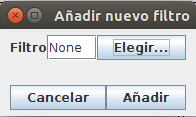
\includegraphics[width=0.5\textwidth]{img/anexo/Filtro_dialog1}
		\caption{Diálogo para la selección de filtro.}\label{fig:img/anexo/Filtro_dialog1}
	\end{figure}
%						\imagen{img/anexo/Filtro_dialog1}{Diálogo para la selección de filtro.}
	\begin{figure}[!h]
		\centering
		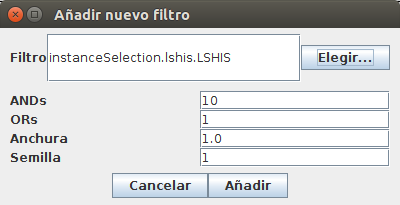
\includegraphics[width=0.7\textwidth]{img/anexo/Filtro_dialog2}
		\caption{Diálogo para la selección de filtro después de seleccionar un algoritmo.}\label{fig:img/anexo/Filtro_dialog2}
	\end{figure}		
						
%									\imagen{img/anexo/Filtro_dialog2}{Diálogo para la selección de filtro después de seleccionar un algoritmo.}
			
			\item \textbf{Panel de selección de clasificador y validación cruzada:} Su funcionalidad es similar a la descrita en paneles anteriores, concretamente el panel de selección de filtro. Sin embargo, es este caso solo es posible añadir un único clasificador (así como solo una única configuración de validación cruzada), por lo que las opciones que típicamente se mostraban en un diálogo separado, ahora se muestran en la propia pantalla (ver imagen \ref{img/anexo/Clasificador_dialog}).
			
									\imagen{img/anexo/Clasificador_dialog}{Panel para la configuración del clasificador y la validación cruzada.}			
			
		\end{itemize}
	\item \textbf{Menú inferior:} Cuenta con dos botones para ejecutar diferentes acciones. La modalidad ``ZIP'' será descrita en la subsección \ref{subsec:createZip}, pero en esta sección nos interesa presionar el botón ``Ejecutar''.
	\end{itemize}
	
Antes de lanzar una ejecución surge la pregunta de cuantas ejecuciones diferentes se han programado. Se generarán tantas ejecuciones como posibles combinaciones entre componentes se puedan crear con las configuraciones propuestas. Así pues, si, por ejemplo, se han indicado dos configuraciones de Spark, dos conjuntos de datos y dos filtros se realizarán $2 \times 2 \times 2 = 8$ ejecuciones, puesto que el clasificador será siempre el mismo.
	
Una vez hemos cumplimentado todos los campos requeridos (los únicos opcionales son los que se refieren a la validación cruzada) y presionamos sobre el botón ``Ejecutar'' veremos como en la esquina inferior izquierda se muestra un nuevo texto indicando la ejecución que se está realizando. Un ejemplo de un experimento completamente configurado y en funcionamiento puede verse en la imagen \ref{fig:img/anexo/Interfaz_completa_rellena}

\imagen{img/anexo/Interfaz_completa_rellena}{Ventana principal de la interfaz gráfica rellena.}

No se pueden lanzar varias baterías de experimentos a la vez, así que si intentásemos crear una nueva ejecución y ejecutarla mientras la anterior continúa funcionando recibiremos un mensaje de error.

Una vez terminadas todas las ejecuciones, la interfaz nos informará de ello mediante un nuevo diálogo. Podemos ir a consultar el resultado en el directorio \textit{results} que se ha generado en la carpeta desde la que hemos lanzado la ejecución. Si hemos iniciado el programa haciendo doble clic sobre el fichero .jar este directorio probablemente se encuentre en la carpeta \$HOME del usuario.

\subsection{Definición de una batería de ejecución y lanzamiento por separado}\label{subsec:createZip}

El procedimiento inicial es similar al marcado en \ref{subsec:ejecutaGUI}, es decir, una vez abierta la interfaz gráfica hemos de indicar todas las configuraciones de ejecución que deseemos. La diferencia esta vez la encontramos al final de la operación, donde en lugar de presionar sobre el botón ``Ejecutar'', lo haremos sobre el botón ``ZIP''

Esta operación, que tal vez puede tardar unos instantes si hemos seleccionado conjuntos de datos muy grandes, generará una carpeta de nombre ``zip'' en el directorio desde donde hemos invocado la interfaz gráfica. Dentro de la carpeta encontraremos un nuevo archivo .zip que contendrá un script de ejecución .sh junto con todos los conjuntos de datos que necesitemos para realizar las ejecuciones que hemos definido previamente.

Ese fichero lo moveremos a donde sea necesario, típicamente un servicio clúster donde se encuentre Spark instalado junto con nuestra librería en el directorio \textit{\$SPARK\_HOME/lib}, tal y como se ha indicado en \ref{subsec:InstalarISAlgorithms}.

Una vez allí, el archivo puede descomprimirse usando el comando: 

\begin{lstlisting}[language=bash]
$ unzip <fichero-zip>
\end{lstlisting}

Es posible que, para descomprimir el archivo necesitemos un paquete \textit{unzip} instalado. Si no existe, podremos obtenerlo con el comando

\begin{lstlisting}[language=bash]
$ sudo apt-get install unzip
\end{lstlisting}

Finalmente, hemos de ejecutar el archivo .sh que acabamos de descomprimir. Para ello, desde consola, podemos movernos a la ruta donde se encuentre el fichero y escribir en terminal:

\begin{lstlisting}[language=bash]
$ chmod +x Bateria_de_Ejecucion.sh
$ ./Bateria_de_Ejecucion.sh
\end{lstlisting}

Deberían comenzar las ejecuciones en Spark, una tras otra, hasta que finalicen todas.

\subsection{Lanzamiento en el servicio Google Cloud Dataproc}

Google Cloud Dataproc es uno de los muchos servicios que ofrece la plataforma Google Cloud (\url{https://cloud.google.com/}). Para acceder a todos ellos es necesario contar con una cuenta Google, cuyo proceso de registro no será descrito en este manual. Igualmente, existen diferentes maneras de utilizar este servicio. En este apartado se describirá únicamente la manera de uso gráfica, por ser la más intuitiva para realizar labores sencillas.

Lo primero que debemos saber es que los servicios ofrecidos en Google Cloud (incluido el propio Google Cloud Dataproc) suelen están asociados a un proyecto concreto, aunque, si acabamos de registrarnos, ya contaremos con un proyecto creado. De querer generar uno nuevo podemos hacerlo en el menú superior, clic sobre el nombre del proyecto actual y clic sobre ``Crear proyecto'' en el menú desplegable que generará la acción anterior (ver imagen \ref{fig:img/anexo/dataproc_crearProyecto}).

\imagen{img/anexo/dataproc_crearProyecto}{Creación de un nuevo proyecto en Google Cloud.}

Es importante indicar que, en el caso de estar realizando esta tarea con la versión de prueba de Google Cloud, no deberemos crear un nuevo proyecto, pues la condición gratuita se aplica solo al proyecto generado por defecto por Google.

Una vez tengamos nuestro proyecto nos encontraremos ante su página de inicio (ver imagen \ref{fig:img/anexo/dataproc_inicio}), aunque no entraremos a explicar el funcionamiento de la misma.

\imagen{img/anexo/dataproc_inicio}{Página de inicio de un proyecto en Google Cloud.}

El segundo paso será almacenar nuestro archivo .jar, junto con los conjuntos de datos, en algún lugar que Google pueda alcanzar. Para ello, lo más sencillo será usar un segundo servicio de Google Cloud: Google Cloud Storage. Podemos acceder a él desde el menú superior, haciendo clic sobre el icono situado más a la izquierda y seleccionando el servicio ``Storage'' de entre las opciones que muestre el menú emergente (ver imagen \ref{fig:img/anexo/dataproc_selectService}).

\imagen{img/anexo/dataproc_selectService}{Menú de selección de servicios de Google Cloud.}

Si el proyecto es nuevo, es posible que tengamos que reservar un nuevo segmento de memoria para poder guardar nuestros datos. Simplemente hacemos clic sobre la opción ``Crear segmento'' que veremos en el centro de nuestra pantalla y rellenamos los campos de ``Nombre'', ``Clase de almacenamiento'' y ``Ubicación'' acorde a nuestras preferencias. Una vez terminado este paso, podemos acceder a nuestro nuevo espacio de memoria y administrarlo según nuestro gusto mediante las opciones del menú superior o arrastrando hacia la ventana del navegador todos aquellos elementos que deseamos que sean subidos al servicio de almacenamiento.

Ahora, necesitar asignar ciertos permisos a nuestro proyecto para poder asignarle un clúster. Para ello, vamos a visitar el servicio ``Compute Engine'' de la misma manera que antes visitamos ``Storage'', presionando el icono de la izquierda en el menú superior y buscando el servicio entre la lista de posibles. Lo primero que se nos preguntará es si deseamos asignar una serie de permisos a nuestro proyecto, a lo cual aceptaremos.

Con todo preparado, vamos a acceder finalmente al servicio que realmente nos interesa: Google Cloud Dataproc. Repetimos la misma operación anterior y buscamos servicio ``Dataproc''.

Ahora, vamos a crear nuestro primer clúster. Presionamos sobre el botón ``Crear nueva agrupación'' que veremos en el centro de la pantalla y rellenamos el formulario que permitirá crear un clúster. Es importante saber que:

\begin{itemize}
\item Es conveniente situar la ubicación del clúster en la misma que el segmento de memoria que está destinado a usar.
\item Si estamos ejecutando desde la versión gratuita de Google Cloud, el tamaño del clúster estará limitado a 8 CPUs, incluyendo el nodo maestro.
\item En el apartado ``Opciones de acceso, inicialización, versión, red, segmento y trabajadores prioritarios'' podemos seleccionar la ``versión de imagen'' del clúster, lo que definirá la versión de los productos que vamos a usar. Este proyecto se ha probado con la versión 0.2 que incluye Spark 1.5.2
\item También en el apartado ``Opciones de acceso, inicialización, versión, red, segmento y trabajadores prioritarios'' hay una opción llamada ``Segmento de aplicación de fases de Cloud Storage''. Aquí debemos indicar el segmento de memoria que hemos creado anteriormente. Si no especificamos nada se creará uno por defecto.
\end{itemize}

\imagen{img/anexo/dataproc_clusterMenu}{Pantalla principal de Google Cloud Dataproc}

Bien, con nuestro clúster creado únicamente falta definir la tarea que debemos ejecutar.
Para ello, en el menú lateral izquierdo podremos ver una sección llamada ``Tareas'' (ver imagen \ref{fig:dataproc_clusterMenu}). Nos podemos dirigir a ella y crear una nueva tarea del mismo modo que hemos creado anteriormente un segmento de memoria o una agrupación. De nuevo, es importante tener en cuenta que:

\begin{itemize}
\item Deberemos definir el ``Tipo de tarea'' como ``Spark''
\item La ruta al archivo .jar (o al fichero que contenga el conjunto de datos cuando introduzcamos las opciones) tendrá una estructura similar a ``gs://nombreSegmento/directorio/fichero'' si hemos utilizado el servicio Google Cloud Dataproc.
\end{itemize}

Podemos ver un ejemplo de una configuración en la imagen \ref{fig:img/anexo/dataproc_tareaConfigurada}.

\imagen{img/anexo/dataproc_tareaConfigurada}{Ejemplo de una tarea configurada}

Lanzada la aplicación seremos redirigidos a una nueva pantalla donde podremos observar una línea de comandos tal y como si hubiésemos  lanzado la aplicación en nuestra propia máquina. Mientras la ejecución tiene lugar podemos realizar cualquier otro tipo de operación, incluido definir nuevas tareas.

Una vez terminada la tarea que hayamos programado, queda ver el fichero resultante de la aplicación, para lo que deberemos conectarnos al nodo maestro. Accedemos a la vista principal de nuestro clúster desde la pantalla principal de Google Dataproc (ver imagen \ref{fig:img/anexo/dataproc_clusterMenu}) y allí hacemos click sobre ``Instancias de VM'' y sobre el botón ``SSH'' que aparecerá junto al nombre del nodo maestro.
Esto abrirá una nueva ventana del navegador que emulará una consola de comandos. No es objetivo de esta sección hablar de todas las posibles opciones que podemos realizar, únicamente veremos el fichero resultante ejecutando el siguiente comando:

\begin{lstlisting}[language=bash]
$ cat /tmp/nombre_tarea/results/nombre_fichero_resultados
\end{lstlisting}

\subsection{Cheatsheet}\label{subsec:cheatsheet}
A continuación se va realizar un listado con todas las posibles opciones que actualmente pueden formar parte de la sentencia de invocación del programa.

 \begin{table}
  \begin{center}
   \begin{tabular}{| m{3cm} | L{9cm} |}
    \hline
    \centering Parámetro &  Descripción \\
    \hline
    \rowcolor{gray}
    \multicolumn{2}{|m{13cm}|}{\centering Tipo de ejecución} \\
    \hline
   	\centering ISClassExec & Define una tarea en la que intervenga un algoritmo de selección de instancias y un clasificador \\
   	\hline
   	\centering ISClassExecTest & Define una tarea en la que intervenga un algoritmo de selección de instancias y un clasificador y, además mide el tiempo de ejecución de la labor de filtrado. Este último modo de lanzamiento podría afectar ligeramente a la ejecución de la tarea, aumentando su tiempo de ejecución. Para más información ver \ref{subsec:}\\
   	\hline
   	\rowcolor{gray}
   	\multicolumn{2}{|m{13cm}|}{\centering Parámetros del lector} \\
   	\hline
   	\centering -f & Indica que el atributo de clase es el primero de los atributos de cada instancia.\\
   	\hline
   	\centering -hl + Int & Indica que existe una cabecera en el fichero y cuantas líneas forman dicha cabecera. \\
   	\hline
   	   	\rowcolor{gray}
   	\multicolumn{2}{|m{13cm}|}{\centering Parámetros para el selector de instancias} \\
   	\hline
   	   	\rowcolor{lightgray}
   	\multicolumn{2}{|m{13cm}|}{\centering instanceSelection.lshis.LSHIS} \\
   	\hline
   	\centering -and + Int & Número de funciones AND.\\
   	\hline
   	\centering -or + Int & Número de funciones OR.\\
   	\hline
   	\centering -w + Double & Anchura de los \textit{buckets}.\\
   	\hline
   	\centering -s + Long & Semilla utilizada para generar números aleatorios.\\
   	\hline
   	\rowcolor{lightgray}
   	\multicolumn{2}{|m{13cm}|}{\centering instanceSelection.demoIS.DemoIS} \\
   	\hline
   	\centering -rep + Int & Número de votaciones a realizar.\\
   	\hline
   	\centering -alpha +  Double & Valor alpha.\\
   	\hline
   	\centering -np +  Int & Número de particiones en las que se dividirá el conjunto de datos original. \\
   	\hline
   	\centering -dsperc + Double & Porcentaje del conjunto de datos utilizado para calcular el error durante el cómputo del fitness. \\
   	\hline
   	\centering -s + Long & Semilla utilizada para generar números aleatorios.\\
   	\hline
   	   	\rowcolor{gray}
   	\multicolumn{2}{|m{13cm}|}{\centering Parámetros para el clasificador} \\
   	\hline
   	   	\rowcolor{lightgray}
   	\multicolumn{2}{|m{13cm}|}{\centering classification.seq.knn.KNN} \\
   	\hline
   	\centering -k + Int & Número de vecinos más cercanos\\
   	\hline

   \end{tabular}
   \caption{Cheatsheet}
   \label{tabla:cheatsheet}
  \end{center}
 \end{table}

\todo{recordar que aquí hay un enlace roto}
